\documentclass{beamer}
\usetheme{metropolis}
\title{Enhancement to the Open edX HTML Editor}
\date{\today}
\author{
	Ashutosh Sathe
	(\texttt{2ashutoshbs@gmail.com}) \\
	\and
	Srijan Roy Choudhury
	(\texttt{roychoudhurysrijan442@gmail.com}) \\
	\and
	Pravallika Podugu
	(\texttt{pravallikapodugu22@gmail.com}) \\
}
\begin{document}

	\maketitle

	\begin{frame}{OpenEdx Overview}
		\begin{block}{What is OpenEdx ?}
			An open source MOOC platform developed by professionals at Harvard and MIT.
			OpenEdx platform consists of modules called XBlocks. In short, EdX platform is "Xblock Runtime"
		\end{block}
		\begin{block}{Main Components : }
			\begin{itemize}
				\item LMS
				\item CMS
				\item Catalog
				\item Analytics
				\item Notes API
				\item Ecommerce
			\end{itemize}
		\end{block}
	\end{frame}
	
	\begin{frame}{ HTML Editor }
		\begin{block}{Why do we need HTML Editor ?}
			\begin{itemize}
				\item Adding content to course
				\item Discussion Forums
				\item Email
			\end{itemize}
		\end{block}
		\begin{block}{Solutions adopted by OpenEdx : }
			\begin{itemize}
				\item TinyMCE : WYSIWYG
				\item CodeMirror : Advanced editor for TinyMCE
				\item WMD : Mainly Email and Discussion Forums
			\end{itemize}
		\end{block}
	\end{frame}
	
	\begin{frame}{Current Senario }
		\begin{block}{Current versions : }
			\begin{itemize}
				\item TinyMCE : 4.0.20
				\item CodeMirror : 3.27
				\item WMD : Unknown version from 2012
			\end{itemize}
		\end{block}
		\begin{block}{Issues : }
			\begin{itemize}
				\item Editors are very old
				\item HTML code is not well indented and it is very hard to edit
				\item Internal CSS is not supported
			\end{itemize}
		\end{block}
	\end{frame}
	
	\begin{frame}{Backend Overview}
		\begin{block}{Technologies}
			\begin{itemize}
				\item \textbf{Python, Django} for web applications
				\item \textbf{MongoDB} database for courses
				\item \textbf{MySQL} for pre-learner data
				\item \textbf{Amazon S3/YouTube} for videos
			\end{itemize}
		\end{block}
	\end{frame}
	
	\begin{frame}{Our approach }
		\begin{block}{Observations}
			\begin{itemize}
				\item Latest version of CodeMirror has good features like code folding, indentation etc.
				\item \textbf{CodeMirror-For-TiynMCE} : A plugin for TinyMCE to replace TinyMCE's raw HTML Editor by CodeMirror
			\end{itemize}
		\end{block}
	\end{frame}
	
	\begin{frame}{Our approach }
		\begin{block}{The indentation problem in raw HTML Editor }
			\begin{itemize}
				\item Download the latest version of TinyMCE , CodeMirror and CodeMirror-For-TinyMCE plugin
				\item Integrate and test the plugin on updated editors
				\item Use this updated editor as raw HTML Editor in OpenEdx system
			\end{itemize}
		\end{block}
		\begin{block}{Expected Result }
			TinyMCE opening the instance of latest codemirror as it's raw HTML editor
		\end{block}
	\end{frame}
	
	\begin{frame}{Our approach }
		\begin{block}{Alternative approach to indentation solution }
			\begin{itemize}
				\item Trying other online editors such as brackets, quill, contenttools
				\item Porting the indentation logic from other editors such as Notepad++ to the current editor
			\end{itemize}
		\end{block}
	\end{frame}
	
	\begin{frame}{Our approach }
		\begin{block}{Supporting internal CSS }
			\begin{itemize}
				\item Wrap the entire HTML content in an iframe
				\item Set the width of iframe to 100\%
				\item Set the height of iframe equal to the height of content of iframe
				\item Set the border of iframe to zero/none
				\item Open all hyperlinks within the iframe in new tab
			\end{itemize}
		\end{block}
		\begin{block}{Expected Result}
			An invisible iframe holdinng our HTML content
		\end{block}
	\end{frame}
	
	\begin{frame}{Our approach }
		\begin{block}{Alternative approach for supporting internal CSS }
			\begin{itemize}
				\item Use javascript to apply CSS
				\item Separate out CSS part from HTML content
				\item Wrap the entire content in a div with unique id
				\item Select each and every child of the div and apply styles to it
			\end{itemize}
		\end{block}
		\begin{block}{Expected Result}
			An invisible iframe holdinng our HTML content
		\end{block}
	\end{frame}
	
	\begin{frame}{Working over Approach \#1}
		\begin{block}{Advantages of Approach \#1 of both the problems}
			\begin{itemize}
				\item Upgrading something is always better than integrating something new altogether
				\item The iframe appraoch also allows the course content creator to include third party CSS such as bootstrap, w3css which will make the course even more beautiful
				\item Wrapping data inside the iframes containerizes the data ensuring no mixing of CSS between 2 HTML blocks in LMS
			\end{itemize}
		\end{block}
	\end{frame}
	
	\begin{frame}{Working over Approach \#1}
		\begin{block}{Steps for completing Approach \#1}
			\begin{itemize}
				\item Download the latest versions of both the editors
				\item Test each editor individually
				\item Integrate both the editors using \textit{codemirror for tinymce} plugin.We call this integration as hybrid version of tinymce
				\item Test this hybrid editor
				\item Integrate this hybrid editor with django(Since EdX uses django as well)
				\item Test this django integration
				\item Set up a working environment of OpenEdx platform
				\item Integrate the hybrid editor with the OpenEdx platform
				\item Testing the complete product
			\end{itemize}
		\end{block}
	\end{frame}
	
	\begin{frame}{Working over Approach \#1}
		\begin{block}{Summary of local django integration}
			\begin{itemize}
				\item Most of the HTML tags and their attributes work
				\item Most of the CSS styles and attributes work
				\item CSS animations and external CSS such as bootstrap works
				\item Report of this integration can be found \alert{\href{https://docs.google.com/spreadsheets/d/1AJQWfAG2NIjpxFZt2fnLPlKdhP2-q35KZ0DOmdb-F0w/edit?ts=5b2744d4\#gid=0}{on link (1)}}
				\item Source code of this integration can be found here \alert{\href{https://github.com/ashutoshbsathe/codemirror-in-tinymce/tree/django-test}{on link (2)}}
				\item Wrapping content inside iframe(for internal CSS) is implemented in django backend(Check source code for more info)
			\end{itemize}
		\end{block}
		\begin{block}{Links :}
			\tiny {\begin{enumerate}[I]
			\item \tiny{\href{https://docs.google.com/spreadsheets/d/1AJQWfAG2NIjpxFZt2fnLPlKdhP2-q35KZ0DOmdb-F0w/edit?ts=5b2744d4\#gid=0}{https://docs.google.com/spreadsheets/d/1AJQWfAG2NIjpxFZt2fnLPlKdhP2-q35KZ0DOmdb-F0w/edit?ts=5b2744d4\#gid=0}}
			\item \tiny{\href{https://github.com/ashutoshbsathe/codemirror-in-tinymce/tree/django-test}{https://github.com/ashutoshbsathe/codemirror-in-tinymce/tree/django-test}}
			\end{enumerate}
			}
		\end{block}
	\end{frame}
	
	\begin{frame}{Working over Approach \#1}
		\begin{block}{Preparing for the integration}
			\begin{itemize}
				\item We keep the TinyMCE at it's same version
				\item We pull our CodeMirror plugin in the \textit{edx-platform/common/statis/js/vendor} \alert{without touching the current CodeMirror folder}
				\item We configure the TinyMCE to use updated CodeMirror
				\item We modify the backend (exact location still unknown) to integrate our CSS solution
			\end{itemize}
		\end{block}
	\end{frame}
	
	\begin{frame}{Working over Approach \#1}
		\begin{block}{Getting a working environment}
			OpenEdx can be installed in one of the following 3 ways
			\begin{itemize}
				\item Devstack
				\item Fullstack
				\item Native Ubuntu Installation
			\end{itemize}
			For developers, as the name suggests, devstack is suggested
		\end{block}
		\begin{block}{Getting a devstack up and running}
			\begin{itemize}
				\item Virtualbox + Vagrant system(Deprecated now)
				\item Docker based system
			\end{itemize}		
		\end{block}
	\end{frame}
	
	\begin{frame}{Getting a working environment}
		\begin{block}{Issues we faced}
			\begin{itemize}
				\item \alert{A LOT OF PROXY CONFIGURATION ISSUES !}
				\item Docker installation and configuration
				\item Building ReactJS assets
				\item Docker container issues
			\end{itemize}
		\end{block}
	\end{frame}
	
	\begin{frame}{Getting a working environment}
		\begin{block}{Dealing with the issues }
			\begin{itemize}
				\item \textbf{Proxy :} Just disable the proxy altogether and use a non-proxy network for downloading everything you need \pause
				\item \textbf{Docker installation : } Follow the steps given on the docker site very very carefully \pause
				\item \textbf{Building ReactJS assets : } Explicitly configure "\textit{babel-loader}" to build JSX \pause
				\item \textbf{Docker container : } Set the environment variables very very carefully and preserve them 
			\end{itemize}
		\end{block}
	\end{frame}
	
	\begin{frame}{Screenshots of working devstack}
		\begin{figure}
			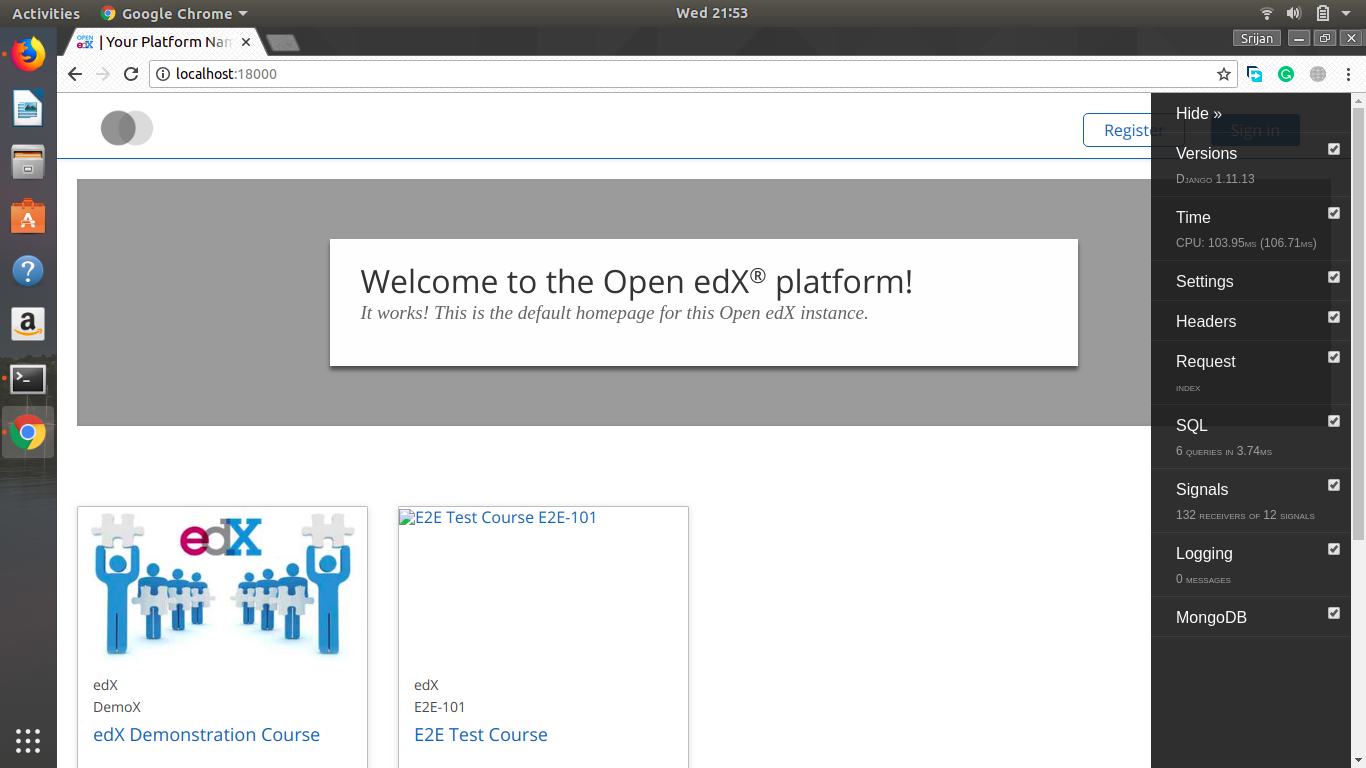
\includegraphics[width=\linewidth,height=\textheight,keepaspectratio]{./18-06-18/devstack-1.png}
		\end{figure}
	\end{frame}
	
	\begin{frame}{Screenshots of working devstack}
		\begin{figure}
			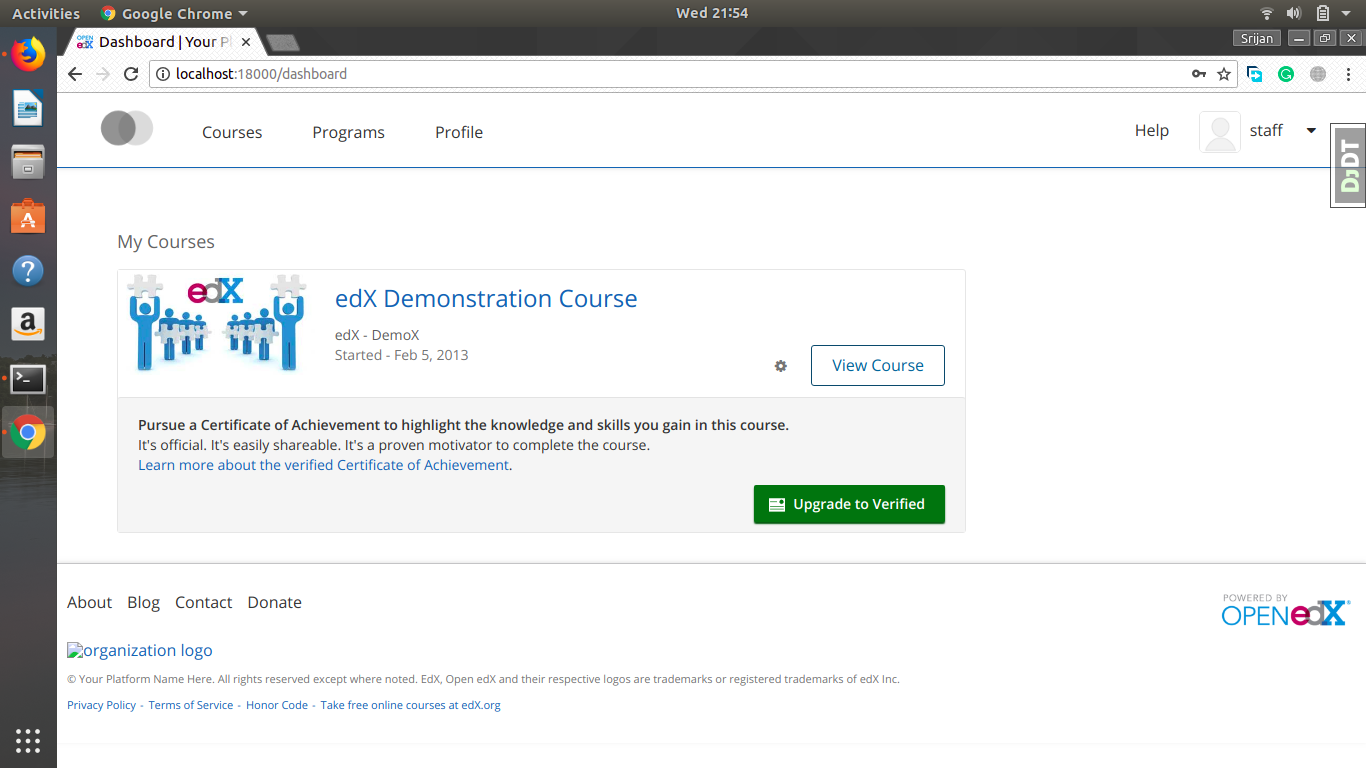
\includegraphics[width=\linewidth,height=\textheight,keepaspectratio]{./18-06-18/devstack-2.png}
		\end{figure}
	\end{frame}
	
	\begin{frame}{Screenshots of working devstack}
		\begin{figure}
			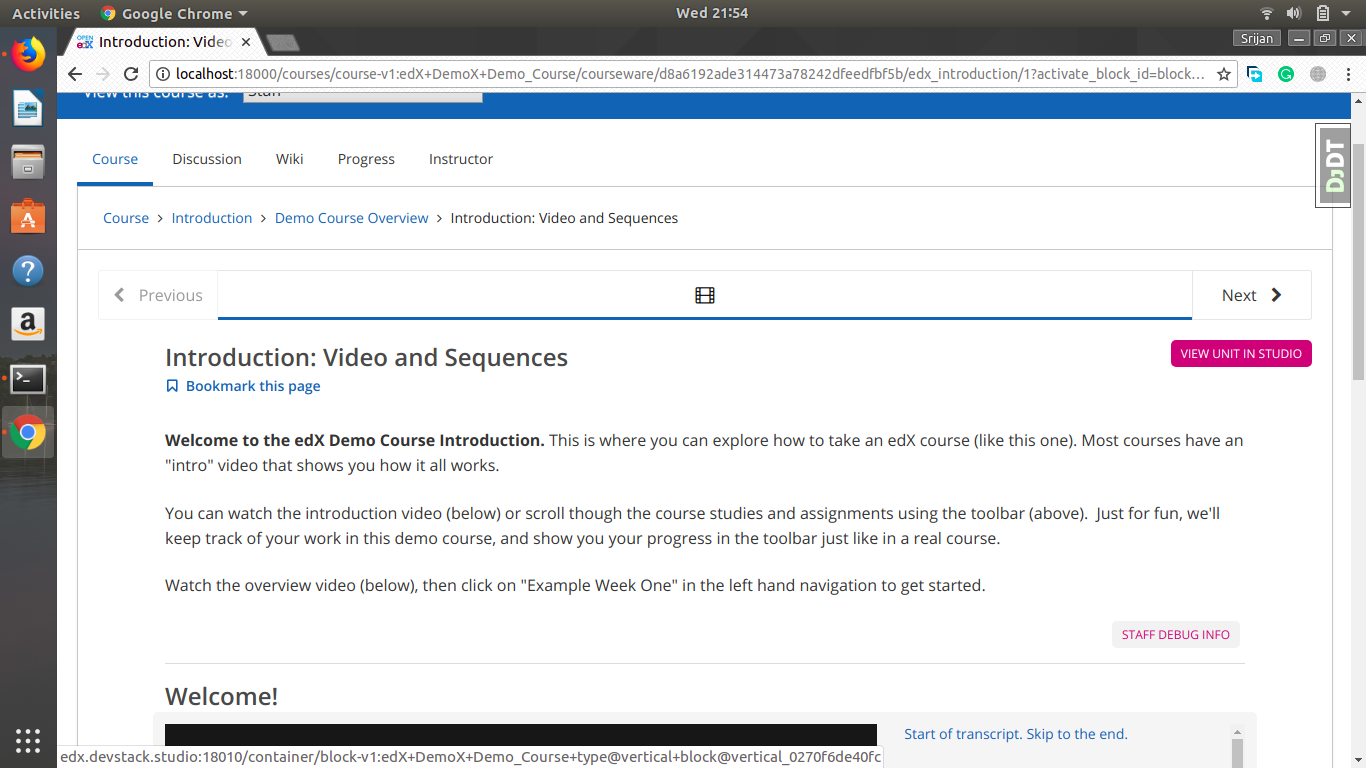
\includegraphics[width=\linewidth,height=\textheight,keepaspectratio]{./18-06-18/devstack-3.png}
		\end{figure}
	\end{frame}
	
	\begin{frame}{Screenshots of working devstack}
		\begin{figure}
			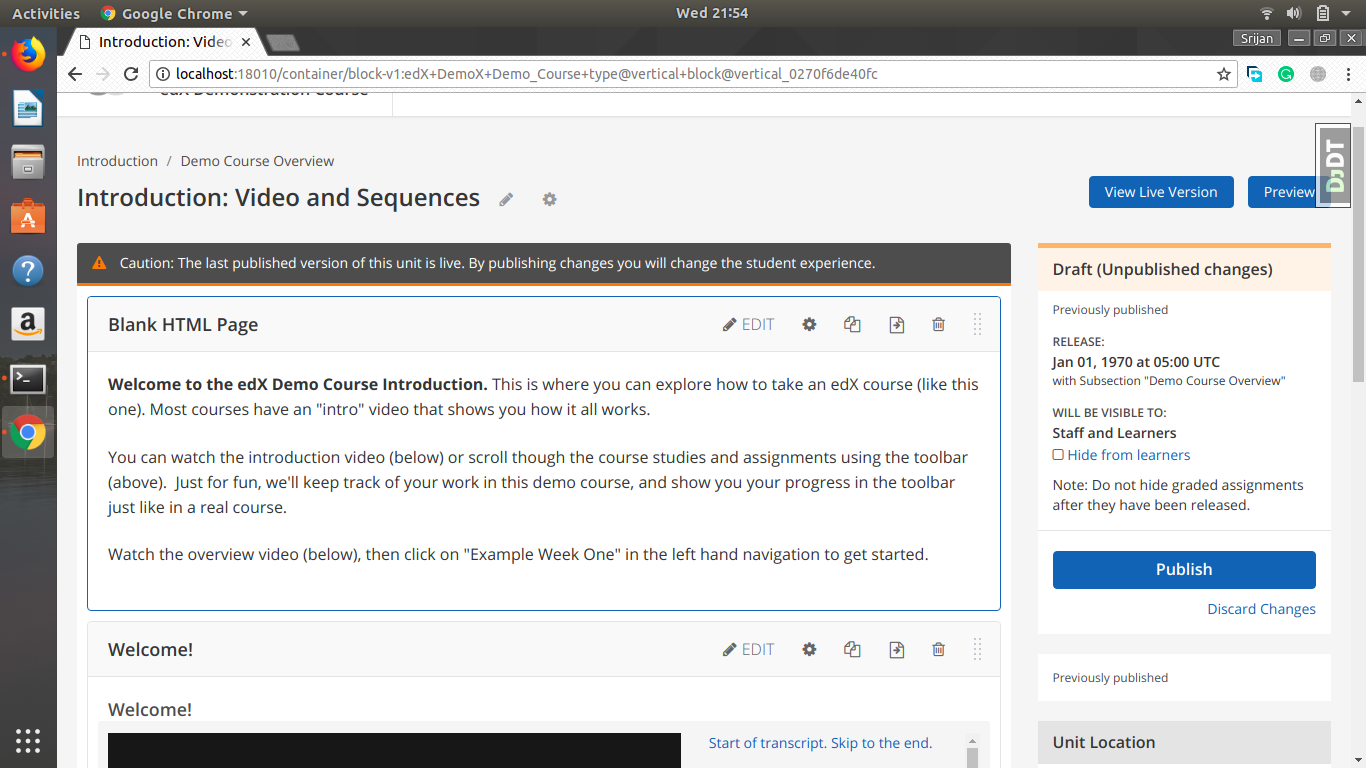
\includegraphics[width=\linewidth,height=\textheight,keepaspectratio]{./18-06-18/devstack-4.png}
		\end{figure}
	\end{frame}
	
	\begin{frame}{Working over Approach \#1}
		\begin{block}{Integrating our hybrid editor with OpenEdx Devstack}
			\begin{itemize}
				\item The work on this is partially done
				\item We were successful in getting the devstack to open updated instance of CodeMirror
				\item The integration source code can be found \alert{\href{https://github.com/ashutoshbsathe/tree/updated-codemirror}{here (1)}}
			\end{itemize}
		\end{block}
		\begin{block}{Issues we face currently :}
			Our CSS styling is not getting saved by OpenEdx backend. We may need to discuss this issue with some backend developer
		\end{block}
		\begin{block}{Links :}
		\tiny{\href{https://github.com/ashutoshbsathe/tree/updated-codemirror}{I. https://github.com/ashutoshbsathe/tree/updated-codemirror}}
		\end{block}
	\end{frame}
	
	\begin{frame}{Conceptual Structure of Devstack}
		\begin{block}{Summary}
			\begin{itemize} \pause
				\item Devstack is a set of services \pause
				\item Each service corresponds to one docker container \pause
				\item Each docker container is made up of docker image and docker volume \pause
				\item Docker images are pulled from OpenEdx repositories 
			\end{itemize}
			\tiny{We also wanted to create a pictorial representation but couldn't do neatly, We will make sure to include that in final documentation}
		\end{block}
	\end{frame}
	
	\begin{frame}{Screenshots of our issues}
		\begin{figure}
			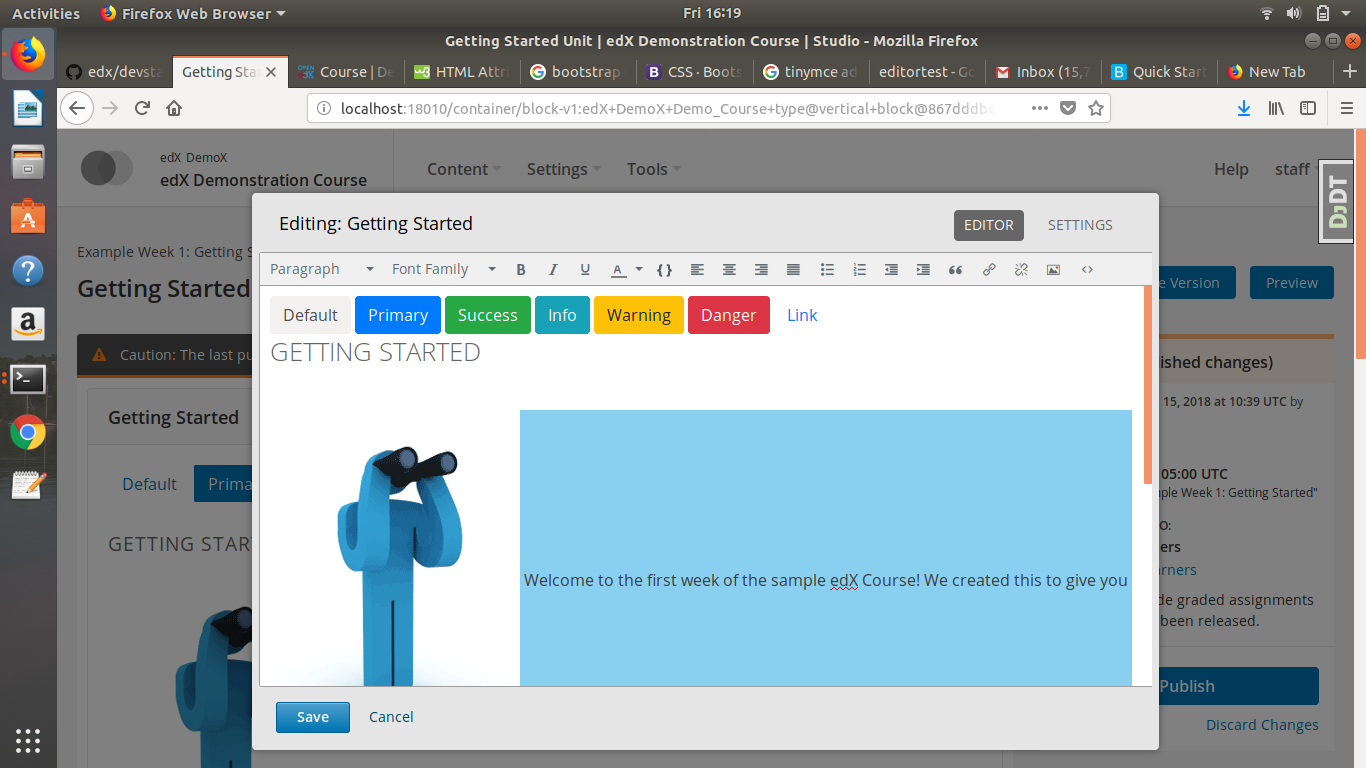
\includegraphics[width=\linewidth,height=\textheight,keepaspectratio]{./18-06-18/issue-1.png}
		\end{figure}
	\end{frame}
	
	\begin{frame}{Screenshots of our issues}
		\begin{figure}
			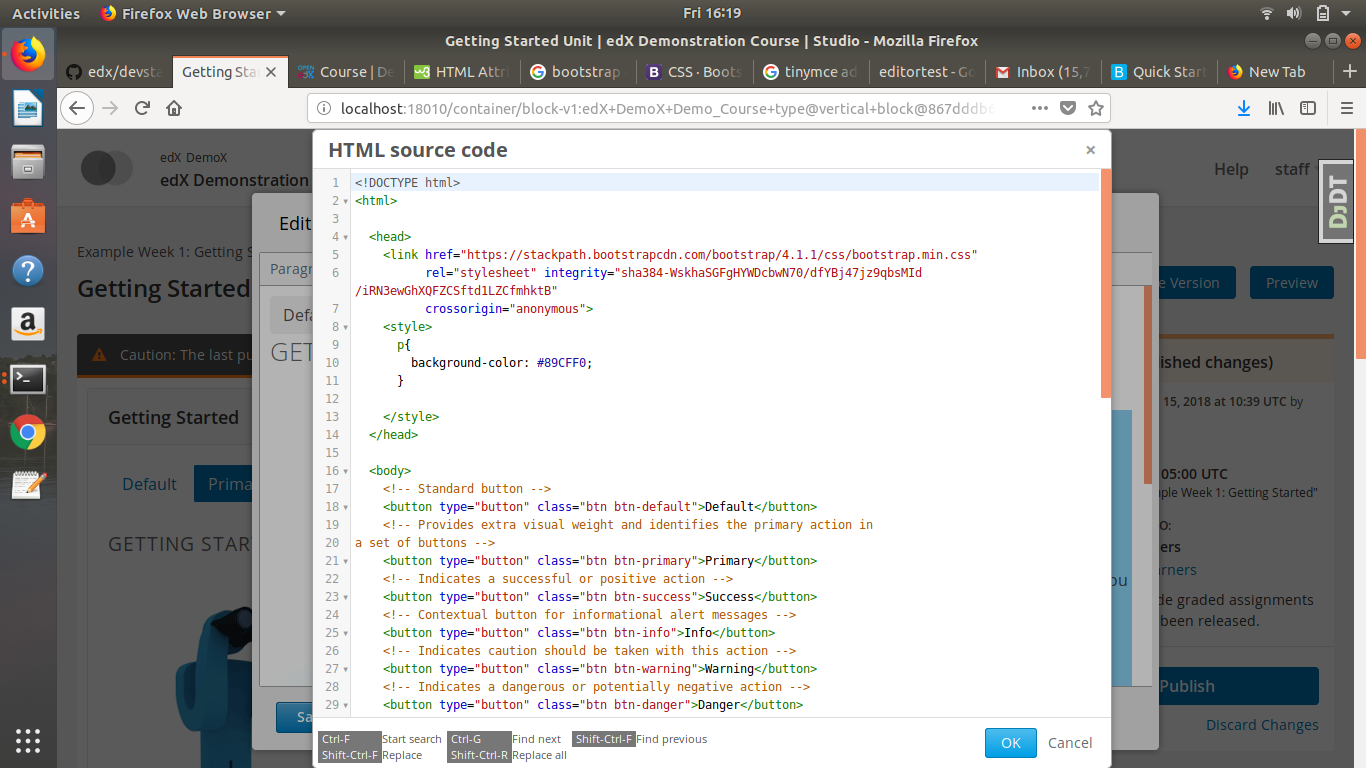
\includegraphics[width=\linewidth,height=\textheight,keepaspectratio]{./18-06-18/issue-2.png}
		\end{figure}
	\end{frame}
	
	\begin{frame}{Screenshots of our issues}
		\begin{figure}
			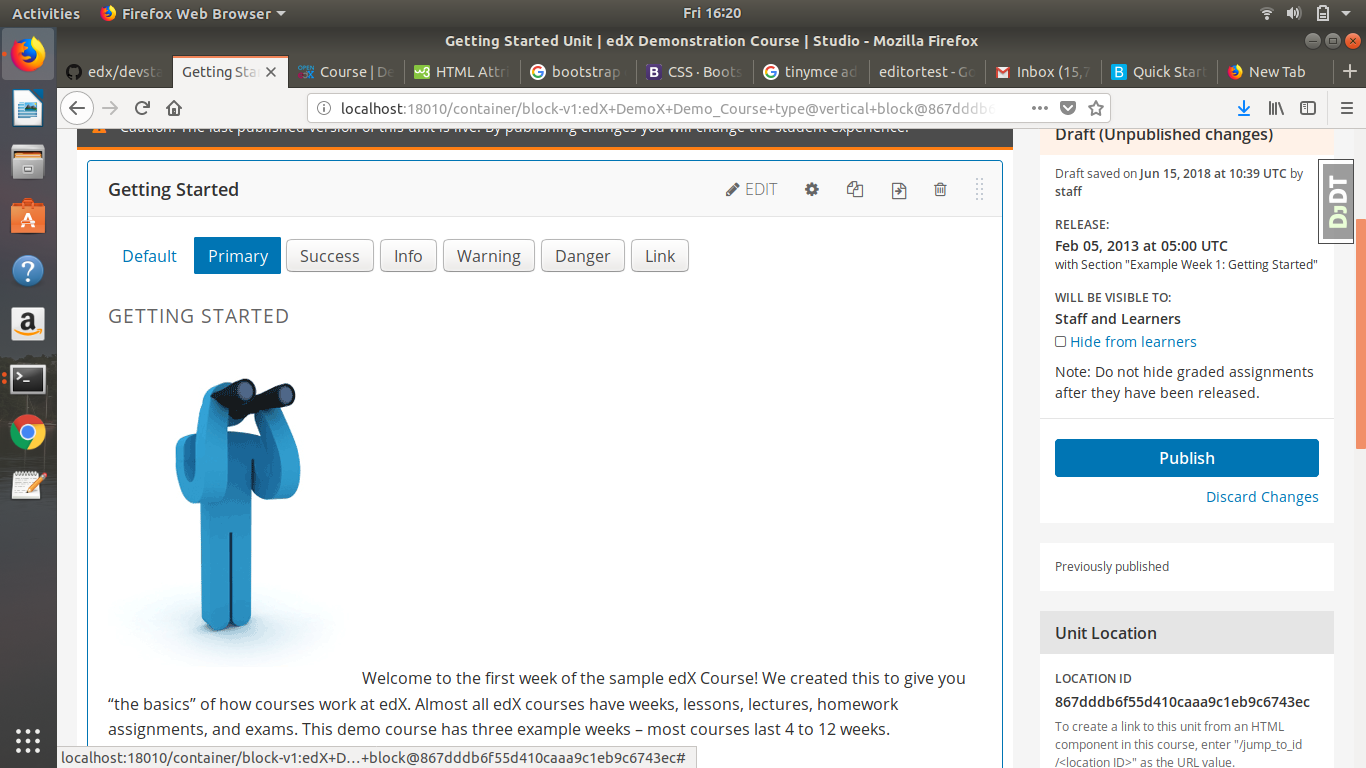
\includegraphics[width=\linewidth,height=\textheight,keepaspectratio]{./18-06-18/issue-3.png}
		\end{figure}
	\end{frame}
	
	\begin{frame}{Working over Approach \#1}
		\begin{block}{Future Work}
			\begin{itemize}
				\item Consult OpenEdX backend developer
				\item Completing the integration of hybrid editor
				\item Rigorous testing of the completed product
				\item Report making
			\end{itemize}
		\end{block}
	\end{frame}
	
	\begin{frame}
		THANK YOU!
	\end{frame}
	
	\begin{frame}
		Questions ?
	\end{frame}

\end{document}
